\subsection{Learning to Rank Algorithms}

In this work, the aim is to look at possibility of ranking the links between Wikipedia articles by their real click-trough rate. Ranking is an essential part of informational retrieval, but not limited to it. It grew even more relevant in recent years when it became important to process large amounts of data in a reasonable amount of time. In order to accomplish this task, we chose to use a family of algorithms called Learning to Rank. These algorithms bring machine learning into information retrieval.

\begin{figure}[H]
    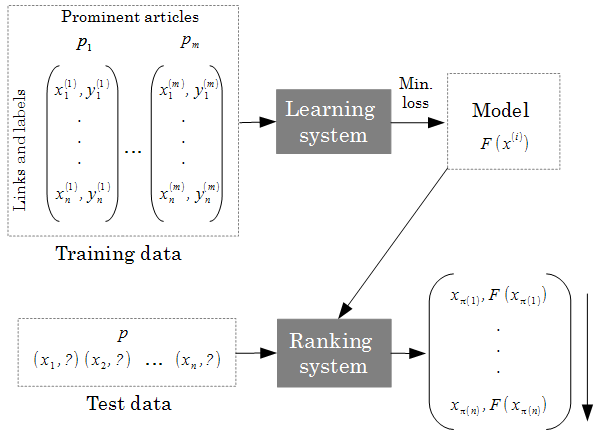
\includegraphics[width=0.49\textwidth]{images/l2r}
 \caption{L2R method}
 \label{fig:l2r}
\end{figure}

\subsubsection{Ranking problem formulation}
Let $p$ be a prominent article and let's denote an associated set of links to article $p$ as $\mathbf{x} = \{x_1, x_2, \ldots, x_m\}$. Every link $x_i$ has its label (relevance evaluation) $y_i$ in the set $\mathbf{y} = \{y_i\}^m_{i=1}$. The values of $y_i$ has to be from some totally ordered set $(S, \le)$.  Ranking can be viewed as a task of finding permutation $\pi$ on indices $\{1,2,\ldots, m\}$ given an article $p$ and its associated set of links $\mathbf{x}$. Permutation $\pi$ must satisfy that $y_{\pi(j)} \le y_{\pi(i)}$ for all $1\le i < j \le m$. The sequence $x_{\pi(1)},x_{\pi(2)}, \ldots, x_{\pi(m)}$ is the ordering of retrieved links according to their relevance in an increasing order with respect to the article $p$.
% * <philip@thruesen.dk> 2016-05-31T21:55:08.397Z:
%
% This section, has a notation describing the same things as in section 2.3 - 3.2 but uses different symbols for the same things like prominent article etc. We have to change one or the other..
%
% ^ <jarekcechak@gmail.com> 2016-06-02T08:04:47.742Z:
%
% no time to fix :-/
%
% ^ <jarekcechak@gmail.com> 2016-06-02T08:05:07.434Z:
%
% just keep in mind for presentation
%
% ^ <jarekcechak@gmail.com> 2016-06-02T08:05:10.572Z.

Learning to rank algorithms handle this task as an instance of a supervised machine learning problem. Each link is represented by its feature vector. Let $p_i$ where $1 \le i \le n$ be the training prominent articles and $\mathbf{x}^{(i)} = \{x_{j}^{(i)}\}_{j = 1}^{m^{(i)}}$ their associated links, where $m^{(i)}$ is the number of links of the article $p_i$. Then $\mathbf{y}^{(i)} = \{y_{j}^{(i)}\}_{j = 1}^{m^{(i)}}$ are labels for the associated links to article $p_i$ (also called ground truth). The set of prominent articles used to train the algorithm is represented by $\mathbf{T} = \{(\mathbf{x}^{(i)},\mathbf{y}^{(i)} )\}_{i = 1}^{n}$. The algorithm then automatically learns a model for $\mathbf{T}$ in the form of a function $F(\mathbf{x}^{(i)})$ that approximates the real mapping $\hat{F}(x^{(i)}) = y^{(i)}$ on the training set. Such model can later be used to predict relevance of new articles outside the training set, where the label is unknown.

The common idea behind creating the model in learning to rank algorithms, or machine learning in general, is optimization of a loss function $L(F(\mathbf{x}^{(i)}), \mathbf{y}^{(i)})$ for $1 \le i \le n$. The loss function describes the quality of the computed ranking in terms of errors made compared to the ground truth. In \cite{LTR4IR} and \cite{li}, the loss function is used to categorize learning to rank algorithms into three groups; pointwise, pairwise, and listwise.

\subsubsection{Pointwise approach}
Pointwise algorithms treat each link (a feature vector to be precise) as an standalone instance. The input for the resulting model is a feature vector and its output is predicted label. Essentially, the problem is simplified to regression, classification, or  ordinal regression as each document is treated independently as a point in the feature space. Loss functions correspond to  regression, classification, or ordinal loss functions. A limitation pointed out in \cite{LTR4IR} assumes relevance is absolute and does not depend on the article.
% * <roelcastanomoreno@gmail.com> 2016-05-31T11:14:24.263Z:
%
% >  A limitation pointed out in \cite{LTR4IR} assumes relevance is absolute and does not depend on the article.
%
% Clarify this sentence
%
% ^ <roelcastanomoreno@gmail.com> 2016-06-02T08:09:12.973Z.

\subsubsection{Pairwise approach}
Pairwise algorithms consider pairs of links. The input for the model is a pair of feature vectors and the output is their relative preference, i.e. if the first from the pair should be ranked higher that the second one or vice versa. The loss function in this approach measures discrepancy between preference predicted by the model and actual order in the ground truth.

\subsubsection{Listwise approach}
Listwise algorithms look at a whole list of documents. The input for the model is a list of feature vectors and the output is either a list of labels or a permutation. This approach is the only one where the loss function directly measures the final position/rank of documents.

\subsubsection{RankLib}
\label{sec:ranklib}
To perform the previously mentioned approaches of Learning to Rank we use the RankLib library \cite{ranklib}, which implements the following algorithms.
\begin{itemize}
\item MART \cite{MART} (pointwise)
\item RankNet \cite{RankNet} (pairwise)
\item RankBoost \cite{RankBoost} (pairwise)
\item AdaRank \cite{AdaRank} (listwise)
\item Coordinate Ascent \cite{CoordinateAscent} (listwise)
\item LambdaMART \cite{LambdaMART} (listwise)
\item ListNet \cite{ListNet} (listwise)
\item Random Forests \cite{RandomForests} (pointwise)
\end{itemize}